% Provenance (never printed): cycle 4 SVT/physique, "La planete Terre,
% l'environnement": the ocean, its relief, its waters and their movements;
% see sources/book1/PROVENANCE.md. Book 1, grade 8, chapter 4.
% Vocabulary guard: owns the parts of the seafloor (one definition),
% salinity, ocean current (homograph: electric current -- link "ocean
% current" only), gyre. Ridge and trench were met as places in g7.1 (plate
% boundaries); seafloor spreading and subduction stay there. The deep
% circulation is told (no "thermohaline" definition: Book 2).
\chapter{महासागर}\label{ch:g8:the-oceans}

दिसंबर 1872 में ब्रिटिश नौसेना का एक जहाज़, HMS \emph{चैलेंजर}, दुनिया भर की साढ़े
तीन वर्ष की यात्रा पर इंग्लैंड से निकला। उसका काम नया था: यह पता करना कि \omterm{def:g2:water-on-earth:ocean}{महासागरों} की
तली में क्या है। बार-बार जहाज़ खुले \omterm{def:g2:water-on-earth:ocean}{समुद्र} में रुकता, और नाविक एक लंबी रस्सी पर एक भारी
वज़न तब तक नीचे उतारते जब तक वह तली को न छू ले; छोड़ी गई रस्सी की लंबाई गहराई देती
थी। जब मई 1876 में जहाज़ घर लौटा, तो उसकी गहराई-मापों ने दिखा दिया था कि \omterm{def:g2:water-on-earth:ocean}{महासागर} की तली
में गहरे \omterm{def:g1:landscapes-around-us:landform}{मैदान} और बड़ी \omterm{def:g1:landscapes-around-us:landform}{पर्वत} शृंखलाएँ हैं।
% ledger: nhm:challenger-voyage, edin:challenger-stations

\begin{omfigure}
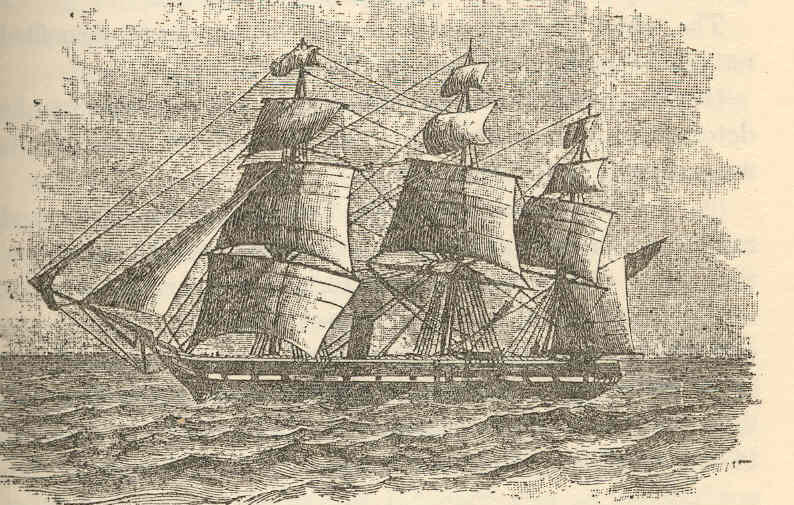
\includegraphics[width=0.55\linewidth]{images/book1/g8-challenger-sounding.jpg}

{\small \omterm{def:g2:water-on-earth:ocean}{महासागर} की गहराई मापने की तैयारी करता HMS \emph{चैलेंजर}, 1872। अभियान की
रिपोर्टों से एक उत्कीर्ण चित्र, जो हर्डमैन की पुस्तक \emph{फ़ाउंडर्स ऑफ़ ओशनोग्राफ़ी}
(1923) में पुनर्मुद्रित है; सार्वजनिक डोमेन, विकिमीडिया कॉमन्स के
ज़रिए।}
% ledger: commons:challenger
\label{fig:g8:the-oceans:challenger}
\end{omfigure}

आज एक जहाज़ ध्वनि से \omterm{def:g2:water-on-earth:ocean}{समुद्र} की तली का \omterm{def:g2:drawing-to-map:map}{मानचित्र} बनाता है। उसके पेंदे के नीचे लगा एक
उपकरण ध्वनि का एक छोटा स्पंद नीचे भेजता है; ध्वनि तली से टकराकर लौटती है और प्रतिध्वनि
के रूप में वापस आती है। प्रतिध्वनि को लगने वाला समय गहराई देता है, बार-बार, जबकि जहाज़
चलता रहता है। यह \emph{सोनार} है।
% ledger: nos:sonar

\begin{recall}
\omterm{def:g2:water-on-earth:salt-fresh}{खारा पानी} पृथ्वी के ज़्यादातर हिस्से को ढकता है, एक ही विश्व \omterm{def:g2:water-on-earth:ocean}{महासागर} में जो \omterm{def:g2:water-on-earth:ocean}{महासागरों}
और \omterm{def:g2:water-on-earth:ocean}{समुद्रों} में बँटा है (\cref{ch:g2:water-on-earth})। \omterm{def:g8:the-oceans:seafloor}{महासागरीय कटकों} पर \omterm{def:g7:plate-tectonics:plate}{प्लेटें} एक-दूसरे
से दूर जाती हैं और खाइयों पर एक \omterm{def:g7:plate-tectonics:plate}{प्लेट} दूसरी के नीचे धँसती है
(\cref{ch:g7:plate-tectonics})। \omterm{def:g2:water-on-earth:ocean}{महासागरों} के ऊपर पवनें बड़ी पेटियों में बहती हैं:
\omterm{def:g8:winds-global-circulation:global-winds}{व्यापारिक पवनें}, \omterm{def:g8:winds-global-circulation:global-winds}{पछुआ पवनें} और \omterm{def:g8:winds-global-circulation:global-winds}{ध्रुवीय पुरवा पवनें}, जिन्हें पृथ्वी का घूमना एक ओर मोड़
देता है (\cref{ch:g8:winds-global-circulation})।
\end{recall}

\section{महासागर की तली}

अगर \omterm{def:g2:water-on-earth:ocean}{महासागरों} का पानी निकाला जा सकता, तो एक पूरा छिपा हुआ \omterm{def:g1:landscapes-around-us:landscape}{भूदृश्य} दिखाई देता। तटों के
साथ-साथ ज़मीन \omterm{def:g2:water-on-earth:ocean}{समुद्र} के नीचे एक हल्की ढलान वाले, उथले चबूतरे के रूप में आगे जाती है।
फिर तली एक खड़ी ढलान से नीचे किलोमीटरों गहरे विशाल, समतल \omterm{def:g1:landscapes-around-us:landform}{मैदानों} तक गिरती है। इन
\omterm{def:g1:landscapes-around-us:landform}{मैदानों} से \omterm{def:g1:landscapes-around-us:landform}{पर्वत} शृंखलाएँ उठती हैं, और जहाँ-तहाँ संकरी खाइयाँ पृथ्वी पर किसी भी दूसरी
चीज़ से ज़्यादा गहरी नीचे जाती
हैं।
% ledger: edin:challenger-stations

\begin{omfigure}
\begin{tikzpicture}[font=\footnotesize, >={Stealth[length=2mm]}]
  \fill[omSea] (0,0) rectangle (15.6,-4.2);
  \fill[omLithAlluv] (0,0.6) -- (1.2,0.15) -- (1.6,0) -- (3.4,-0.35)
    .. controls (3.9,-0.55) and (4.1,-2.6) .. (4.7,-3.1)
    -- (6.6,-3.35) -- (7.6,-3.1) -- (8.3,-2.2) -- (8.6,-1.7) -- (8.75,-1.9) -- (8.9,-1.65) -- (9.2,-2.3) -- (10.0,-3.15)
    -- (11.6,-3.4) -- (12.6,-3.45) -- (13.05,-4.1) -- (13.35,-3.0) -- (14.2,-0.9) -- (14.8,0.7) -- (15.6,1.3)
    -- (15.6,-4.6) -- (0,-4.6) -- cycle;
  \draw[black!70] (0,0.6) -- (1.2,0.15) -- (1.6,0) -- (3.4,-0.35)
    .. controls (3.9,-0.55) and (4.1,-2.6) .. (4.7,-3.1)
    -- (6.6,-3.35) -- (7.6,-3.1) -- (8.3,-2.2) -- (8.6,-1.7) -- (8.75,-1.9) -- (8.9,-1.65) -- (9.2,-2.3) -- (10.0,-3.15)
    -- (11.6,-3.4) -- (12.6,-3.45) -- (13.05,-4.1) -- (13.35,-3.0) -- (14.2,-0.9) -- (14.8,0.7) -- (15.6,1.3);
  \draw[omRiver] (1.55,0) -- (14.45,0);
  \node[anchor=south] at (8,0.05) {समुद्र तल};
  \node[align=center] at (2.6,-0.85) {महाद्वीपीय\\मग्नतट};
  \draw[->] (2.6,-0.55) -- (2.6,-0.25);
  \node[align=center, anchor=east] at (3.7,-2.0) {महाद्वीपीय\\ढाल};
  \draw[->] (3.75,-2.0) -- (4.1,-1.9);
  \node[align=center] at (5.7,-2.6) {वितलीय मैदान};
  \node[align=center] at (8.75,-0.9) {महासागरीय कटक};
  \draw[->] (8.75,-1.15) -- (8.75,-1.55);
  \node[align=center] at (11.1,-2.6) {वितलीय मैदान};
  \node[align=center, anchor=west] at (13.5,-3.9) {महासागरीय\\खाई};
  \draw[->] (13.45,-3.9) -- (13.15,-3.9);
  \node[anchor=south] at (0.8,0.6) {महाद्वीप};
  \node[anchor=south east] at (14.7,1.0) {पर्वत};
\end{tikzpicture}

{\small \omterm{def:g2:water-on-earth:ocean}{महासागर} की तली के हिस्से, एक \omterm{def:g1:landscapes-around-us:water}{तट} से खुले \omterm{def:g2:water-on-earth:ocean}{महासागर} तक और दूसरे \omterm{def:g1:landscapes-around-us:water}{तट} तक (एक रेखाचित्र:
गहराइयाँ और चौड़ाइयाँ पैमाने पर नहीं हैं)।}
\label{fig:g8:the-oceans:sketch}
\end{omfigure}

\begin{definition}[महासागर की तली के हिस्से]\label{def:g8:the-oceans:seafloor}
\begin{itemize}
  \item \emph{महाद्वीपीय मग्नतट}\index{महाद्वीपीय मग्नतट} किसी \omterm{def:g3:continents-and-oceans:continent}{महाद्वीप} का \omterm{def:g2:water-on-earth:ocean}{समुद्र} के
        नीचे का उथला, हल्की ढलान वाला किनारा है।
  \item \emph{महाद्वीपीय ढाल}\index{महाद्वीपीय ढाल} वह खड़ी ढलान है जो मग्नतट से
        नीचे गहरी महासागरीय तली तक ले जाती है।
  \item \emph{वितलीय मैदान}\index{वितलीय मैदान} \omterm{def:g2:water-on-earth:ocean}{महासागर} की तली का एक विशाल, बहुत
        समतल और गहरा हिस्सा है।
  \item \emph{महासागरीय कटक}\index{महासागरीय कटक} \omterm{def:g2:water-on-earth:ocean}{समुद्र} के नीचे के \omterm{def:g1:landscapes-around-us:landform}{पर्वतों} की एक
        लंबी शृंखला है जो वितलीय \omterm{def:g1:landscapes-around-us:landform}{मैदानों} से उठती है।
  \item \emph{महासागरीय खाई}\index{महासागरीय खाई} \omterm{def:g2:water-on-earth:ocean}{महासागर} की तली में एक लंबा, संकरा
        और बहुत गहरा गर्त है, जो अक्सर \omterm{def:g1:landscapes-around-us:landform}{पर्वतों} या \omterm{def:g4:volcanoes-earthquakes-first-look:volcano}{ज्वालामुखी} द्वीपों की किसी शृंखला के
        बगल में होता है।
\end{itemize}
\end{definition}
% ledger: edin:challenger-stations, usgs:trench-depth

\omterm{def:g2:water-on-earth:ocean}{महासागर} औसतन लगभग \qty{3700}{m} गहरा है, जो ज़मीन के सबसे ऊँचे \omterm{def:g1:landscapes-around-us:landform}{पर्वत} की ऊँचाई का
लगभग आधा है। उसका सबसे गहरा बिंदु, प्रशांत \omterm{def:g2:water-on-earth:ocean}{महासागर} में मारियाना खाई का चैलेंजर गर्त,
सतह से लगभग \qty{11000}{m} नीचे
है।
% ledger: nos:ocean-depth, usgs:trench-depth, tht:everest


\begin{method}[महासागर की तली का प्रोफ़ाइल पढ़ना]
\begin{enumerate}
  \item अक्ष पढ़ो: आड़े दूरी, ऊपर-नीचे ऊँचाई या गहराई, और ऊर्ध्वाधर
        अतिरंजन।
  \item \omterm{def:g4:world-physical-map:altitude}{समुद्र तल} (ऊँचाई 0) ढूँढो और वे \omterm{def:g1:landscapes-around-us:water}{तट} जहाँ प्रोफ़ाइल उसे पार करता
        है।
  \item किसी \omterm{def:g1:landscapes-around-us:water}{तट} से तली के साथ चलो: उथला मग्नतट, खड़ी ढाल, फिर गहरे समतल
        \omterm{def:g1:landscapes-around-us:landform}{मैदान}।
  \item देखो कि \omterm{def:g1:landscapes-around-us:landform}{मैदानों} से क्या ऊपर उठता है (एक कटक) या उनसे नीचे गिरता है (एक
        खाई), और उसकी गहराई पढ़ो।
\end{enumerate}
\end{method}

\begin{example}[दक्षिण अटलांटिक के आर-पार]
ऊपर वाले प्रोफ़ाइल पर, दक्षिण अमेरिका के \omterm{def:g1:landscapes-around-us:water}{तट} के आगे, तली \qty{3000}{m} से ज़्यादा
गहराई तक गिर जाती है, \qty{300}{km} से भी कम दूरी में। \omterm{def:g8:the-oceans:seafloor}{वितलीय मैदान}, \qty{3500}{m} और \qty{5000}{m} के बीच गहरे, चौड़ाई का ज़्यादातर
हिस्सा भरते हैं। आधे रास्ते पर, प्रोफ़ाइल के साथ लगभग \qty{4400}{km} पर, मध्य-अटलांटिक
कटक सतह से लगभग \qty{2300}{m} नीचे तक उठता है: \omterm{def:g1:landscapes-around-us:landform}{मैदानों} से \qty{2000}{m} से ज़्यादा
ऊपर, \omterm{def:g2:water-on-earth:ocean}{समुद्र} के नीचे छिपी एक \omterm{def:g1:landscapes-around-us:landform}{पर्वत} शृंखला। तली के अफ़्रीका की ओर चढ़ने से पहले \omterm{def:g1:landscapes-around-us:landform}{मैदान} फिर
से \qty{5000}{m} से ज़्यादा गहरे हो जाते हैं।
\end{example}
% ledger: data:etopo1 (figdata/grade-8/seafloor_profile.py: ridge crest -2329 m at 4407 km; deepest -5295 m)

\begin{omfigure}
\begin{tikzpicture}
\begin{axis}[omsection, scale only axis, width=14cm, height=3.6cm, xmin=0, xmax=7569,
  ymin=-6000, ymax=1500, ytick={-6000,-4000,-2000,0}, xtick={0,1000,...,7000},
  xlabel={30.5\textdegree\ दक्षिण के साथ दूरी, 59.5\textdegree\ पश्चिम से (km)}, ylabel={ऊँचाई (m)},
  tick label style={font=\scriptsize}, label style={font=\small},
  yticklabel style={/pgf/number format/1000 sep={\,}}, xticklabel style={/pgf/number format/1000 sep={\,}},
  axis background/.style={fill=white}, clip=true]
  \fill[omSea] (axis cs:0,-6000) rectangle (axis cs:7569,0);
  \addplot[fill=omLithAlluv, draw=black!70, line width=0.5pt] table[x=km, y=elev_m] {figdata/out/grade-8-seafloor_profile-atlantic-rock.dat};
  \node[font=\scriptsize, align=center, fill=white, inner sep=1pt] at (axis cs:4407,-900) {मध्य-अटलांटिक कटक};
  \draw[-{Stealth[length=1.5mm]}] (axis cs:4407,-1250) -- (axis cs:4407,-2150);
  \node[font=\scriptsize] at (axis cs:2500,-5300) {वितलीय मैदान};
  \node[font=\scriptsize] at (axis cs:6200,-5600) {वितलीय मैदान};
  \node[font=\scriptsize, anchor=south west] at (axis cs:30,350) {दक्षिण अमेरिका};
  \node[font=\scriptsize, anchor=south east] at (axis cs:7380,350) {अफ़्रीका};
  \node[anchor=north] at (rel axis cs:0.75,0.97) {\omve{260}};
\end{axis}
\end{tikzpicture}

\medskip
\begin{tikzpicture}
\begin{axis}[omsection, scale only axis, width=7cm, height=3.6cm, xmin=0, xmax=3020,
  ymin=-6000, ymax=4500, ytick={-6000,-4000,-2000,0,2000,4000}, xtick={0,1000,2000,3000},
  xlabel={20.5\textdegree\ दक्षिण के साथ दूरी (km)}, ylabel={ऊँचाई (m)},
  tick label style={font=\scriptsize}, label style={font=\small},
  yticklabel style={/pgf/number format/1000 sep={\,}}, xticklabel style={/pgf/number format/1000 sep={\,}},
  axis background/.style={fill=white}, clip=true]
  \fill[omSea] (axis cs:0,-6000) rectangle (axis cs:3020,0);
  \addplot[fill=omLithAlluv, draw=black!70, line width=0.5pt] table[x=km, y=elev_m] {figdata/out/grade-8-seafloor_profile-pacific-rock.dat};
  \node[font=\scriptsize, align=center, fill=white, inner sep=1pt] at (axis cs:1300,1600) {पेरू--चिली खाई};
  \draw[-{Stealth[length=1.5mm]}] (axis cs:1750,1150) -- (axis cs:1870,-5000);
  \node[font=\scriptsize, anchor=west] at (axis cs:2600,3500) {एंडीज़};
  \node[font=\scriptsize] at (axis cs:700,-5300) {वितलीय मैदान};
  \node[anchor=north west] at (rel axis cs:0.01,0.98) {\omve{148}};
\end{axis}
\end{tikzpicture}

{\small \omterm{def:g2:water-on-earth:ocean}{महासागर} की तली के दो असली प्रोफ़ाइल, ETOPO1 उच्चावच से \omterm{def:g6:latitude-longitude:longitude}{देशांतर} के हर डिग्री पर
पढ़े गए। ऊपर: दक्षिण अटलांटिक के आर-पार, दक्षिण अमेरिका से अफ़्रीका तक। नीचे: दक्षिण
अमेरिका के प्रशांत किनारे के आर-पार। ऊँचाइयों को दूरियों की तुलना में 260 और 148 गुना
खींचा गया है (\emph{ऊर्ध्वाधर अतिरंजन}), नहीं तो \omterm{def:g2:water-on-earth:ocean}{महासागर} काग़ज़ की एक शीट जितना पतला
दिखता; और हर डिग्री पर एक बिंदु होने से संकरी खाई असल से कम गहरी
दिखती है।}
% ledger: data:etopo1, earth:Rmean (figdata/grade-8/seafloor_profile.py)
\label{fig:g8:the-oceans:profiles}
\end{omfigure}


\section{खारा पानी}

\omterm{def:g2:water-on-earth:ocean}{समुद्र} का पानी खारा लगता है क्योंकि उसमें लवण घुले हैं। उनमें से ज़्यादातर \omterm{def:g3:continents-and-oceans:continent}{महाद्वीपों} की
\omterm{def:g3:stones-pebbles-sand:rock}{चट्टानों} से आते हैं: वर्षा \omterm{def:g3:stones-pebbles-sand:rock}{चट्टानों} को धीरे-धीरे घिसती है और \omterm{def:g1:landscapes-around-us:water}{नदियाँ} उनके घुले हुए लवण
\omterm{def:g2:water-on-earth:ocean}{समुद्र} तक ले जाती हैं। कुछ \omterm{def:g2:water-on-earth:ocean}{महासागर} की तली के गरम सोतों से आते
हैं।
% ledger: nos:salinity-varies

\begin{definition}[लवणता]\label{def:g8:the-oceans:salinity}
समुद्री पानी की \emph{लवणता}\index{लवणता} एक किलोग्राम समुद्री पानी में घुले लवणों
का द्रव्यमान है। औसतन यह लगभग \qty{35}{g} प्रति किलोग्राम है: समुद्री पानी के
द्रव्यमान का \qty{3.5}{\%}
लवण है।
\end{definition}
% ledger: nos:salinity-varies

\omterm{def:g8:the-oceans:salinity}{लवणता} हर जगह एक जैसी नहीं है। जब समुद्री पानी भाप बनकर उड़ता है, तो पानी चला जाता है
पर लवण पीछे रह जाते हैं: जहाँ धूप तेज़ है और वर्षा दुर्लभ, वहाँ \omterm{def:g2:water-on-earth:ocean}{समुद्र} ज़्यादा खारा हो
जाता है। जहाँ बहुत वर्षा होती है, या जहाँ कोई बड़ी \omterm{def:g1:landscapes-around-us:water}{नदी} आकर मिलती है, वहाँ \omterm{def:g2:water-on-earth:ocean}{समुद्र} कम खारा
होता है। जब समुद्री पानी जमकर समुद्री बर्फ़ बनता है, तो लवण आसपास के पानी में रह जाता है,
जो भी ज़्यादा खारा हो जाता है। कुल मिलाकर, \omterm{def:g8:the-oceans:salinity}{लवणता} \omterm{def:g3:continents-and-oceans:equator}{भूमध्य रेखा} के पास, जहाँ बहुत वर्षा
होती है, और \omterm{def:g3:continents-and-oceans:poles}{ध्रुवों} के पास कम है; वह मध्य \omterm{def:g6:latitude-longitude:latitude}{अक्षांशों} में, \ang{30} के पास की सूखी
पेटियों के नीचे, सबसे ज़्यादा है।
% ledger: nos:salinity-varies, nos:sea-ice-salt, mo:three-cells

\begin{omfigure}
\begin{tikzpicture}[font=\footnotesize, >={Stealth[length=2mm]}]
  \fill[omSea] (0,0) rectangle (13,-1.6);
  \draw[omRiver, line width=0.8pt] (0,0) -- (13,0);
  % left: dry belt, evaporation
  \fill[yellow!80!orange] (1.2,3.0) circle (0.35);
  \foreach \x in {1.0,1.8,2.6,3.4} \draw[->, black!50, line width=0.9pt, decorate, decoration={snake, amplitude=0.6mm, segment length=3mm}] (\x,0.15) -- (\x,1.6);
  \node[align=center] at (2.3,2.2) {तेज़ वाष्पीकरण,\\थोड़ी वर्षा};
  \node[align=center, fill=white, inner sep=1.5pt] at (2.3,-0.8) {\textbf{ज़्यादा खारा}};
  % middle: rain
  \fill[black!20] (5.2,2.9) ellipse [x radius=1.3, y radius=0.4];
  \foreach \x in {4.4,4.8,...,6.0} \draw[omRiver] (\x,2.45) -- (\x-0.2,0.25);
  \node[align=center, fill=white, inner sep=1.5pt] at (5.2,-0.8) {\textbf{कम खारा}};
  \node at (5.2,3.55) {भारी वर्षा};
  % right: river mouth and sea ice
  \fill[omLithAlluv] (7.4,0) -- (9.6,0) -- (9.6,0.6) -- (7.4,0.35) -- cycle;
  \draw[omRiver, line width=2pt, ->] (9.4,0.45) -- (7.9,0.2);
  \node[anchor=south] at (8.6,0.65) {नदी};
  \node[align=center, fill=white, inner sep=1.5pt] at (8.6,-0.8) {\textbf{कम खारा}};
  \fill[white, draw=omCold] (10.6,0.25) -- (12.6,0.25) -- (12.4,-0.25) -- (10.8,-0.25) -- cycle;
  \node[anchor=south] at (11.6,0.3) {समुद्री बर्फ़ बनती है};
  \node[align=center, fill=white, inner sep=1.5pt] at (11.6,-0.95) {\textbf{ज़्यादा खारा}\\(लवण पीछे छूटता है)};
\end{tikzpicture}

{\small \omterm{def:g2:water-on-earth:ocean}{समुद्र} की \omterm{def:g8:the-oceans:salinity}{लवणता} को क्या बदलता है: वाष्पीकरण और जमना लवणों को पीछे छोड़ देते हैं;
वर्षा और \omterm{def:g1:landscapes-around-us:water}{नदियाँ} \omterm{def:g2:water-on-earth:salt-fresh}{मीठा पानी} जोड़ती हैं।}
% ledger: nos:salinity-varies, nos:sea-ice-salt
\label{fig:g8:the-oceans:salinity}
\end{omfigure}

\begin{omfigure}
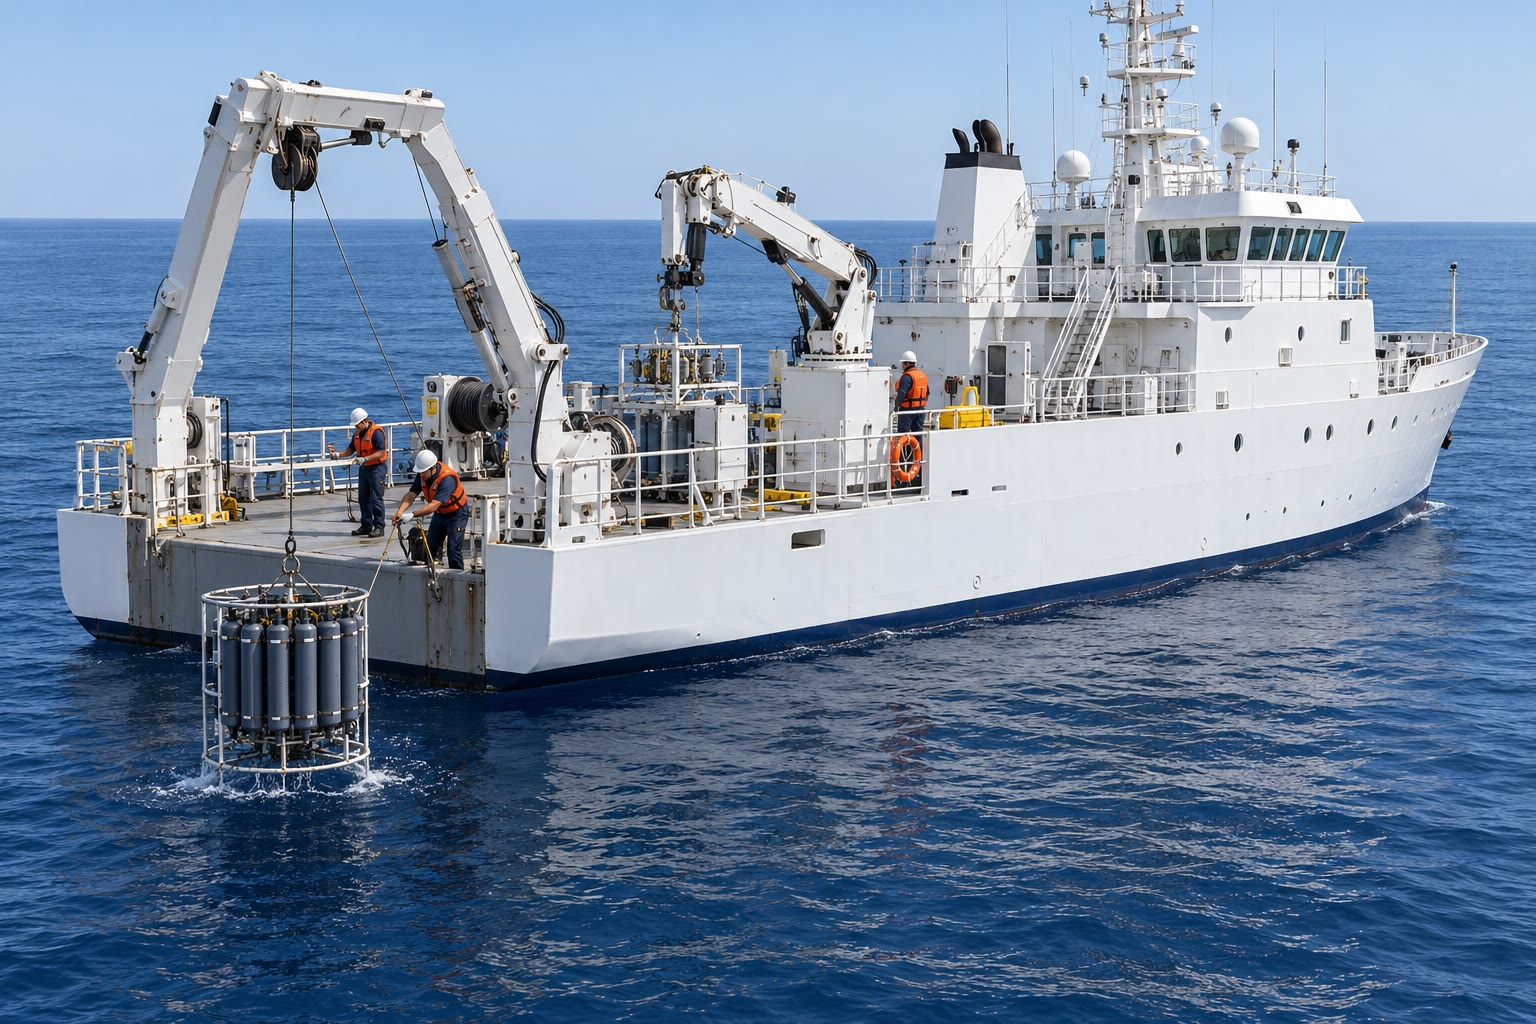
\includegraphics[width=0.58\linewidth]{images/book1/ai/g8-research-ship.jpg}

{\small एक शोध जहाज़ नमूने की बोतलों का एक ढाँचा \omterm{def:g2:water-on-earth:ocean}{समुद्र} में उतारता है, ताकि गहराइयों से
पानी लाकर उसका खारापन और उसका तापमान मापा जा सके (एक सामान्य दृश्य का AI
चित्रण)।}
\label{fig:g8:the-oceans:ship}
\end{omfigure}

\section{सतह की धाराएँ}

\omterm{def:g2:water-on-earth:ocean}{महासागर} कभी शांत नहीं रहता। पवनें उसकी सतह को खींचती हैं और पानी को चला देती हैं: स्थिर
\omterm{def:g8:winds-global-circulation:global-winds}{व्यापारिक पवनें} उसे \omterm{def:g3:continents-and-oceans:equator}{भूमध्य रेखा} के पास पश्चिम की ओर धकेलती हैं, और \omterm{def:g8:winds-global-circulation:global-winds}{पछुआ पवनें} उसे मध्य
\omterm{def:g6:latitude-longitude:latitude}{अक्षांशों} में पूर्व की ओर धकेलती हैं। पवनों की तरह, चलता पानी भी पृथ्वी के घूमने से एक
ओर मुड़ जाता है: \omterm{def:g3:continents-and-oceans:equator}{उत्तरी गोलार्ध} में दाईं ओर, \omterm{def:g3:continents-and-oceans:equator}{दक्षिणी गोलार्ध} में बाईं
ओर।
% ledger: nos:gyres

\begin{definition}[महासागरीय धारा और वलय]\label{def:g8:the-oceans:current}
\emph{महासागरीय धारा}\index{महासागरीय धारा} समुद्री पानी की एक दिशा में स्थिर गति
है, \omterm{def:g2:water-on-earth:ocean}{महासागर} में एक \omterm{def:g1:landscapes-around-us:water}{नदी} की तरह। \emph{वलय}\index{वलय (महासागर)} महासागरीय धाराओं का
एक बहुत बड़ा घेरा है जो किसी महासागरीय द्रोणी के चारों ओर घूमता
है।
\end{definition}
% ledger: nos:gyre-def, nos:gyres
\phantomsection\label{def:g8:the-oceans:gyre}

पाँच बड़े \omterm{def:g8:the-oceans:current}{वलय} हैं: उत्तर और दक्षिण अटलांटिक में, उत्तर और दक्षिण प्रशांत में, और हिंद
\omterm{def:g2:water-on-earth:ocean}{महासागर} में। \omterm{def:g3:continents-and-oceans:equator}{उत्तरी गोलार्ध} के \omterm{def:g8:the-oceans:current}{वलय} दक्षिणावर्त घूमते हैं, \omterm{def:g3:continents-and-oceans:equator}{दक्षिणी गोलार्ध} के वामावर्त।
हर \omterm{def:g2:water-on-earth:ocean}{महासागर} के पश्चिमी किनारे पर \omterm{def:g8:the-oceans:current}{वलय} की धारा संकरी और तेज़ होती है; पूर्वी किनारे पर
वह चौड़ी और धीमी होती
है।
% ledger: nos:gyres

\begin{inthelab}[तश्तरी में एक वलय]
घर के अंदर, एक बड़ी गोल तश्तरी में पानी भरो और सतह पर एक चुटकी काली मिर्च छिड़को।
एक स्ट्रॉ से तश्तरी के आर-पार धीरे-धीरे और लगातार फूँको, हमेशा एक ही दिशा में, एक
किनारे के पास। काली मिर्च देखो: सतह के पास का पानी तुम्हारी साँस के साथ चलने लगता है,
और जल्दी ही पूरी सतह तश्तरी के चारों ओर एक घेरे में घूमने लगती
है।
\end{inthelab}

\begin{omfigure}
\begin{tikzpicture}
\begin{axis}[ommap, width=\linewidth, xmin=-180, xmax=180, ymin=-65, ymax=70,
  xtick={-180,-120,...,180}, ytick={-60,-30,0,30,60},
  xticklabels={$180^\circ$,$120^\circ$\,प,$60^\circ$\,प,$0^\circ$,$60^\circ$\,पू,$120^\circ$\,पू,$180^\circ$},
  yticklabels={$60^\circ$\,द,$30^\circ$\,द,$0^\circ$,$30^\circ$\,उ,$60^\circ$\,उ},
  tick label style={font=\scriptsize}]
  \addplot[fill=omLithAlluv, draw=black!45, line width=0.2pt] table {figdata/out/shared-geo-land.dat};
  \addplot[omWarm, line width=1.3pt] table {figdata/out/grade-8-ocean_currents-gyres-warm.dat};
  \addplot[omCold, line width=1.3pt] table {figdata/out/grade-8-ocean_currents-gyres-cold.dat};
  \addplot[quiver={u=\thisrow{u}, v=\thisrow{v}}, -{Stealth[length=2.6mm, width=2.2mm]}, omWarm, line width=1.3pt]
    table[x=lon, y=lat] {figdata/out/grade-8-ocean_currents-heads-warm.dat};
  \addplot[quiver={u=\thisrow{u}, v=\thisrow{v}}, -{Stealth[length=2.6mm, width=2.2mm]}, omCold, line width=1.3pt]
    table[x=lon, y=lat] {figdata/out/grade-8-ocean_currents-heads-cold.dat};
  \node[font=\scriptsize\bfseries, fill=white, inner sep=1pt, anchor=east] at (axis cs:-72,40) {गल्फ़ स्ट्रीम};
  \node[font=\scriptsize\bfseries, fill=white, inner sep=1pt, anchor=west] at (axis cs:-12,25) {कैनरी धारा};
\end{axis}
\end{tikzpicture}

{\small पाँच बड़े \omterm{def:g8:the-oceans:current}{वलय}, सरल रूप में: \omterm{def:g3:continents-and-oceans:equator}{उत्तरी गोलार्ध} में दक्षिणावर्त, दक्षिणी में
वामावर्त। लाल: गरम धाराएँ, जो \omterm{def:g5:weather-and-climate:tropics}{उष्णकटिबंध} से आती हैं; नीला: ठंडी धाराएँ, जो ऊँचे
\omterm{def:g6:latitude-longitude:latitude}{अक्षांशों} से आती हैं। उत्तर अटलांटिक \omterm{def:g8:the-oceans:current}{वलय} के पश्चिम में गल्फ़ स्ट्रीम और पूर्व में कैनरी
धारा है।}
% ledger: nos:gyres, data:ne-land (figdata/grade-8/ocean_currents.py)
\label{fig:g8:the-oceans:gyres}
\end{omfigure}

इन धाराओं में सबसे प्रसिद्ध गल्फ़ स्ट्रीम है। वह मैक्सिको की खाड़ी से निकलती है, फ़्लोरिडा
के \omterm{def:g1:landscapes-around-us:water}{तट} के साथ-साथ उत्तर की ओर बहती है, उत्तरी कैरोलिना के सामने पूर्व की ओर मुड़ती है और
उत्तर-पूर्व की ओर अटलांटिक पार करती है। उसका गरम पानी औसतन लगभग \qty{6.4}{km} प्रति
घंटा, सतह पर लगभग \qty{9}{km} प्रति घंटा तक, चलता है, और वह दुनिया की सारी \omterm{def:g1:landscapes-around-us:water}{नदियों} से
मिलाकर भी ज़्यादा पानी ले जाती है। वह फ़्लोरिडा के पूर्वी \omterm{def:g1:landscapes-around-us:water}{तट} को जाड़े में गरम रखती है और
पश्चिमी यूरोप तक हल्की गरम हवा लाती
है।
% ledger: nos:gulf-stream, nos:gyres

\begin{omfigure}
\begin{minipage}[c]{0.5\linewidth}\centering
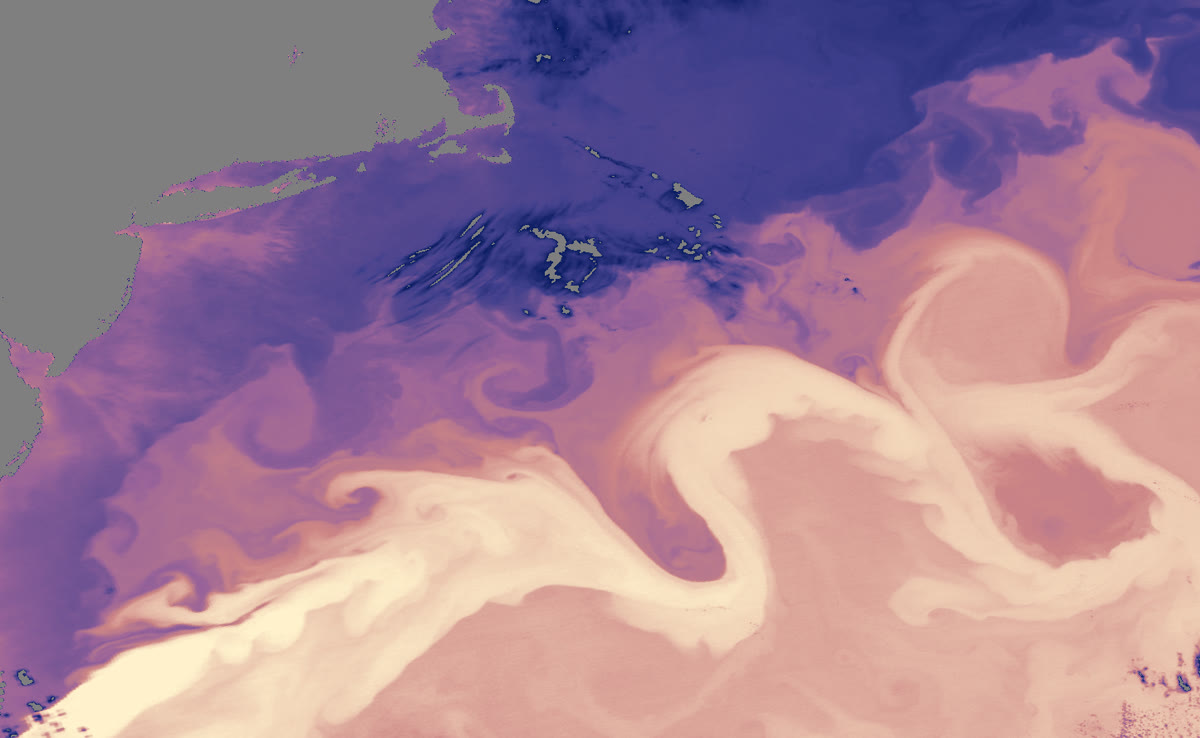
\includegraphics[width=\linewidth]{images/book1/g8-gulf-stream-sst.jpg}
\end{minipage}\hfill
\begin{minipage}[c]{0.46\linewidth}\raggedright
{\small उत्तर अमेरिका के पूर्वी \omterm{def:g1:landscapes-around-us:water}{तट} के सामने \omterm{def:g2:water-on-earth:ocean}{समुद्र} की सतह का तापमान, जिसे NASA के उपग्रह
एक्वा ने 18~अप्रैल 2005 को मापा। गल्फ़ स्ट्रीम गरम पानी की वह पट्टी है (हल्के रंग, लगभग
\qty{23}{\degreeCelsius} तक) जो नीचे बाईं ओर से दाईं ओर बल खाती जाती है, ठंडे पानी
(गहरे रंग, लगभग \qty{-1}{\degreeCelsius} तक) के बीच; ज़मीन धूसर है। NASA (सार्वजनिक
डोमेन, विकिमीडिया कॉमन्स के
ज़रिए)।}
\end{minipage}
% ledger: commons:gulf-sst
\label{fig:g8:the-oceans:gulf}
\end{omfigure}


\section{गहरी धाराएँ और महासागर की ऊष्मा}

पवनें सतह की धाराओं को चलाती हैं। बहुत नीचे, गहरे \omterm{def:g2:water-on-earth:ocean}{महासागर} के ठंडे अँधेरे में, पानी भी
चलता है, कहीं ज़्यादा धीरे। सुदूर उत्तर अटलांटिक में गल्फ़ स्ट्रीम का लाया गरम पानी
अपनी ऊष्मा ठंडी हवा को दे देता है; ठंडा होकर, और समुद्री बर्फ़ बनने पर ज़्यादा खारा
होकर, वह ज़्यादा घना हो जाता है और तली तक डूब जाता है। यह ठंडा, \omterm{def:g2:water-on-earth:salt-fresh}{खारा पानी} \omterm{def:g2:water-on-earth:ocean}{महासागर} की
तली के साथ-साथ दक्षिण की ओर, अंटार्कटिका तक, फिर हिंद और प्रशांत \omterm{def:g2:water-on-earth:ocean}{महासागरों} में रेंगता
है, जहाँ वह धीरे-धीरे ऊपर उठता है और सतह पर लौटता है। पानी की एक बूँद को इस बड़े
चक्कर, \emph{वैश्विक महासागरीय वाहक पट्टी}, का एक पूरा चक्कर लगाने में लगभग
\num{1000} वर्ष लग सकते
हैं।
% ledger: nos:conveyor, nos:sea-ice-salt

\begin{omfigure}
\begin{tikzpicture}
\begin{axis}[ommap, width=\linewidth, xmin=-180, xmax=180, ymin=-65, ymax=70,
  xtick={-180,-120,...,180}, ytick={-60,-30,0,30,60},
  xticklabels={$180^\circ$,$120^\circ$\,प,$60^\circ$\,प,$0^\circ$,$60^\circ$\,पू,$120^\circ$\,पू,$180^\circ$},
  yticklabels={$60^\circ$\,द,$30^\circ$\,द,$0^\circ$,$30^\circ$\,उ,$60^\circ$\,उ},
  tick label style={font=\scriptsize}]
  \addplot[fill=omLithAlluv, draw=black!45, line width=0.2pt] table {figdata/out/shared-geo-land.dat};
  \addplot[omWarm, line width=1.3pt] table {figdata/out/grade-8-conveyor-surface.dat};
  \addplot[omCold, line width=1.3pt, dashed] table {figdata/out/grade-8-conveyor-deep.dat};
  \addplot[quiver={u=\thisrow{u}, v=\thisrow{v}}, -{Stealth[length=2.6mm, width=2.2mm]}, omWarm, line width=1.3pt]
    table[x=lon, y=lat] {figdata/out/grade-8-conveyor-heads-surface.dat};
  \addplot[quiver={u=\thisrow{u}, v=\thisrow{v}}, -{Stealth[length=2.6mm, width=2.2mm]}, omCold, line width=1.3pt]
    table[x=lon, y=lat] {figdata/out/grade-8-conveyor-heads-deep.dat};
  \node[font=\scriptsize\bfseries, fill=white, inner sep=1pt, anchor=west] at (axis cs:4,64) {डूबता है};
  \node[font=\scriptsize\bfseries, fill=white, inner sep=1pt, anchor=south] at (axis cs:163,11) {उठता है};
\end{axis}
\end{tikzpicture}

{\small वैश्विक महासागरीय वाहक पट्टी, एक अकेले चक्कर के रूप में सरल की गई (एक
रेखाचित्र)। लाल: सतह पर गरम पानी; नीला, टूटी रेखा: गहरी महासागरीय तली के साथ-साथ
रेंगता ठंडा, \omterm{def:g2:water-on-earth:salt-fresh}{खारा पानी}। पानी सुदूर उत्तर अटलांटिक में, ग्रीनलैंड और नॉर्वे के बीच,
डूबता है, और प्रशांत में (और, जो नहीं बनाया गया, हिंद \omterm{def:g2:water-on-earth:ocean}{महासागर} में) ऊपर
उठता है।}
% ledger: nos:conveyor, data:ne-land (figdata/grade-8/conveyor.py)
\end{omfigure}

\begin{example}[गहरा पानी कितना धीमा है?]\label{ex:g8:the-oceans:deep-speed}
\omterm{def:g2:drawing-to-map:map}{मानचित्र} पर बना चक्कर मोटे तौर पर \qty{70000}{km} लंबा है। अगर पानी की एक बूँद को उसका
चक्कर लगाने में लगभग \num{1000} वर्ष लगते हैं, तो वह औसतन लगभग
$\num{70000} \div \num{1000} = \qty{70}{km}$ प्रति वर्ष चलती है, यानी लगभग
\qty{200}{m} प्रति दिन। गल्फ़ स्ट्रीम, \qty{6.4}{km} प्रति घंटा पर, एक दिन में लगभग
\qty{150}{km} तय करती है: वह लगभग 11 घंटों में उतनी दूर जाती है जितना गहरा पानी एक
पूरे वर्ष में।
% ledger: nos:conveyor, nos:gulf-stream, earth:Rmean (loop length and speeds computed in figdata/grade-8/conveyor.py)
\end{example}

सतह और गहरी धाराएँ मिलकर ऊष्मा ले जाती हैं: गरम पानी \omterm{def:g5:weather-and-climate:tropics}{उष्णकटिबंध} से \omterm{def:g3:continents-and-oceans:poles}{ध्रुवों} की ओर बहता
है, और ठंडा पानी वापस \omterm{def:g3:continents-and-oceans:equator}{भूमध्य रेखा} की ओर बहता है। पवनों की तरह, \omterm{def:g2:water-on-earth:ocean}{महासागर} सूर्य से पृथ्वी
के असमान गरम होने को बराबर करता
है।
% ledger: nos:conveyor, nos:gulf-stream, mo:global-circ

\section{अभ्यास}

\begin{exercise}[$\star$]\label{exo:g8:the-oceans:1}
\omterm{def:g2:water-on-earth:ocean}{महासागर} की तली के इन हिस्सों को उस क्रम में रखो जिसमें कोई पनडुब्बी किसी \omterm{def:g1:landscapes-around-us:water}{तट} से अटलांटिक
के बीच की ओर जाते हुए उनसे मिलती है: \omterm{def:g8:the-oceans:seafloor}{वितलीय मैदान}; \omterm{def:g8:the-oceans:seafloor}{महाद्वीपीय ढाल}; \omterm{def:g8:the-oceans:seafloor}{महासागरीय कटक};
\omterm{def:g8:the-oceans:seafloor}{महाद्वीपीय मग्नतट}।
\end{exercise}

\begin{exercise}[$\star$]\label{exo:g8:the-oceans:2}
सही या ग़लत? ग़लत वाक्यों को सुधारो। (क) \omterm{def:g2:water-on-earth:ocean}{महासागर} औसतन लगभग \qty{37}{km} गहरा है।
(ख) \omterm{def:g3:continents-and-oceans:equator}{उत्तरी गोलार्ध} के \omterm{def:g8:the-oceans:current}{वलय} दक्षिणावर्त घूमते हैं। (ग) वाष्पीकरण समुद्री पानी को कम खारा
बनाता है। (घ) गल्फ़ स्ट्रीम एक गरम धारा
है।
\end{exercise}

\begin{exercise}[$\star$]\label{exo:g8:the-oceans:3}
हर वर्णन के लिए शब्द बताओ: (क) \omterm{def:g2:water-on-earth:ocean}{समुद्र} के नीचे \omterm{def:g1:landscapes-around-us:landform}{पर्वतों} की एक लंबी शृंखला; (ख) एक
किलोग्राम समुद्री पानी में लवण का द्रव्यमान; (ग) \omterm{def:g8:the-oceans:current}{महासागरीय धाराओं} का एक बहुत बड़ा घेरा;
(घ) \omterm{def:g2:water-on-earth:ocean}{महासागर} की तली में एक लंबा, संकरा और बहुत गहरा
गर्त।
\end{exercise}

\begin{exercise}[$\star$]\label{exo:g8:the-oceans:4}
\omterm{def:g8:the-oceans:current}{वलयों} के \omterm{def:g2:drawing-to-map:map}{मानचित्र} पर: (क) दक्षिण अटलांटिक का \omterm{def:g8:the-oceans:current}{वलय} किस ओर घूमता है? (ख) उत्तर अटलांटिक
की एक गरम धारा और एक ठंडी धारा का नाम बताओ। (ग) कौन-सी पवनें \omterm{def:g3:continents-and-oceans:equator}{भूमध्य रेखा} के पास पानी
को पश्चिम की ओर धकेलती हैं?
\end{exercise}

\begin{exercise}[$\star\star$]\label{exo:g8:the-oceans:5}
\qty{1}{kg} समुद्री पानी के एक नमूने में \qty{35}{g} लवण हैं। (क) उसके द्रव्यमान का
कितना प्रतिशत लवण है? (ख) इस पानी के \qty{20}{kg} में कितने ग्राम लवण हैं? (ग) कितने
किलोग्राम समुद्री पानी में \qty{1}{kg} लवण होते
हैं?
\end{exercise}

\begin{exercise}[$\star\star$]\label{exo:g8:the-oceans:6}
एक जहाज़ का सोनार ध्वनि का एक स्पंद सीधे नीचे भेजता है। प्रतिध्वनि \qty{6}{s} बाद
लौटती है। समुद्री पानी में ध्वनि हर सेकंड लगभग \qty{1500}{m} चलती है। (क) \qty{6}{s}
में ध्वनि कितनी दूर जाती है? (ख) गहराई इस दूरी की केवल आधी क्यों है? (ग) गहराई क्या
है? (घ) जहाज़ \omterm{def:g2:water-on-earth:ocean}{महासागर} की तली के किस हिस्से के ऊपर हो सकता
है?
\end{exercise}

\begin{exercise}[$\star\star$]\label{exo:g8:the-oceans:7}
दक्षिण अटलांटिक के आर-पार वाले प्रोफ़ाइल का उपयोग करो। (क) \omterm{def:g8:the-oceans:seafloor}{वितलीय मैदान} मोटे तौर पर
कितने गहरे हैं? (ख) प्रोफ़ाइल के साथ किस दूरी पर मध्य-अटलांटिक कटक का शिखर है, और वह
कितना गहरा है? (ग) कटक \omterm{def:g1:landscapes-around-us:landform}{मैदानों} से कितने मीटर ऊपर उठता है? (घ) प्रोफ़ाइल को ऊर्ध्वाधर
अतिरंजन की ज़रूरत क्यों है?
\end{exercise}

\begin{exercise}[$\star\star$]\label{exo:g8:the-oceans:8}
\omterm{def:g2:water-on-earth:ocean}{समुद्र} A दो \omterm{def:g5:weather-and-climate:desert}{मरुस्थलों} के बीच है: वहाँ लगभग कभी वर्षा नहीं होती और कोई बड़ी \omterm{def:g1:landscapes-around-us:water}{नदी} उसमें
नहीं गिरती। \omterm{def:g2:water-on-earth:ocean}{समुद्र} B, एक वर्षा वाले क्षेत्र में, बहुत-सी बड़ी \omterm{def:g1:landscapes-around-us:water}{नदियाँ} पाता है। समझाओ कि
दोनों में से कौन खुले \omterm{def:g2:water-on-earth:ocean}{महासागर} से ज़्यादा खारा है, और कौन कम खारा। ये शब्द इस्तेमाल
करो: \emph{वाष्पीकरण}, \emph{\omterm{def:g2:water-on-earth:salt-fresh}{मीठा पानी}}, \emph{लवण पीछे रह
जाते हैं}।
\end{exercise}

\begin{exercise}[$\star\star$]\label{exo:g8:the-oceans:9}
फ़्लोरिडा के \omterm{def:g1:landscapes-around-us:water}{तट} के सामने \omterm{def:g2:water-on-earth:ocean}{समुद्र} में एक बोतल में बंद संदेश फेंका जाता है। (क) पहले कौन-सी
धारा उसे ले जाती है, और किस दिशा में? (ख) फिर वह अटलांटिक को किस ओर पार करती है?
(ग) अगर वह \omterm{def:g8:the-oceans:current}{वलय} के चारों ओर चलती रहती, तो किस \omterm{def:g1:landscapes-around-us:water}{तट} के साथ-साथ दक्षिण की ओर जाती?
(घ) यह धारा गरम है या ठंडी?
\end{exercise}

\begin{exercise}[$\star\star$]\label{exo:g8:the-oceans:10}
गल्फ़ स्ट्रीम औसतन लगभग \qty{6.4}{km} प्रति घंटा चलती है। (क) एक दिन में उसका पानी
कितनी दूर जाता है? (ख) एक सप्ताह में? (ग) \qty{5}{km} प्रति घंटा चलते एक व्यक्ति
से तुलना करो।
\end{exercise}

\begin{exercise}[$\star\star\star$]\label{exo:g8:the-oceans:11}
\omterm{def:g2:water-on-earth:ocean}{महासागर} औसतन लगभग \qty{3700}{m} गहरा है, और उसका सबसे गहरा बिंदु लगभग
\qty{11000}{m} गहरा है। (क) दोनों गहराइयाँ किलोमीटर में लिखो। (ख) सबसे गहरा बिंदु
औसत से कितने गुना गहरा है? एक दशमलव स्थान तक पूर्णांकित करो। (ग) सबसे गहरे बिंदु से
एक सोनार प्रतिध्वनि: \qty{1500}{m} प्रति सेकंड पर, लौटने में कितने सेकंड लगते हैं?
(घ) वाहक पट्टी के पानी की एक बूँद उत्तर अटलांटिक में डूबती है। अगर उसे चक्कर लगाने में
लगभग \num{1000} वर्ष लगते हैं, तो दस की घातों में यह कितने वर्ष
है?
\end{exercise}

\begin{exercise}[$\star\star\star$]\label{exo:g8:the-oceans:12}
गहरे \omterm{def:g2:water-on-earth:ocean}{महासागर} की बड़ी वाहक पट्टी नॉर्वेजियन सागर में, नॉर्वे के \omterm{def:g1:landscapes-around-us:water}{तट} के सामने, शुरू होती है,
जहाँ गल्फ़ स्ट्रीम का लाया गरम पानी अपनी ऊष्मा ठंडी हवा को देता है। (क) \omterm{def:g8:the-oceans:current}{वलयों} के
\omterm{def:g2:drawing-to-map:map}{मानचित्र} और अध्याय का उपयोग करके क़दम-दर-क़दम समझाओ कि यह गरम पानी \omterm{def:g5:weather-and-climate:tropics}{उष्णकटिबंध} से वहाँ
कैसे पहुँचा, और किन पवनों ने उसे धकेला। (ख) समझाओ कि फिर पानी क्यों डूबता है। (ग) वह
आगे कहाँ जाता
है?
\end{exercise}

\section{समस्या: एक बहता हुआ प्लव}

\begin{problem}[{सप्ताहांत समस्या --- फ़्लोरिडा के सामने एक बहता हुआ प्लव छोड़ा जाता है
और उत्तर अटलांटिक वलय के चारों ओर ले जाया जाता है; उसकी यात्रा हिस्सा-दर-हिस्सा देखी
जाती है, और एक चक्कर लगाने में लगने वाला समय निकाला जाता है}]
\label{pb:g8:the-oceans:1}
% ledger: nos:drifter, nos:gulf-stream, nos:gyres (figdata/grade-8/ocean_currents.py; the leg lengths are rounded, the speeds of legs B to D are exercise data)
वैज्ञानिक फ़्लोरिडा के \omterm{def:g1:landscapes-around-us:water}{तट} के सामने एक बहता हुआ प्लव छोड़ते हैं। वह सतह के ठीक नीचे
तैरता है, धाराओं के साथ चलता है, और अपनी स्थिति एक उपग्रह को भेजता है। उसकी बैटरियाँ
लगभग एक वर्ष चलती हैं। \omterm{def:g2:drawing-to-map:map}{मानचित्र} उत्तर अटलांटिक \omterm{def:g8:the-oceans:current}{वलय} के चारों ओर उसकी यात्रा के चार
हिस्से दिखाता है।

\begin{center}
\begin{tikzpicture}
\begin{axis}[ommap, width=11.5cm, xmin=-95, xmax=0, ymin=5, ymax=55,
  xtick={-90,-60,-30,0}, ytick={10,30,50},
  xticklabels={$90^\circ$\,प,$60^\circ$\,प,$30^\circ$\,प,$0^\circ$},
  yticklabels={$10^\circ$\,उ,$30^\circ$\,उ,$50^\circ$\,उ},
  tick label style={font=\scriptsize}]
  \addplot[fill=omLithAlluv, draw=black!45, line width=0.2pt] table {figdata/out/shared-geo-land.dat};
  \addplot[black, line width=1pt, densely dashed, postaction={decorate, decoration={markings,
      mark=between positions 0.04 and 0.98 step 0.08 with {\arrow{Stealth[length=2mm]}}}}]
    table[x=lon, y=lat] {figdata/out/grade-8-ocean_currents-buoy.dat};
  \addplot[only marks, mark=*, mark size=2.2pt, omDef] coordinates {(-79.5,26)};
  \node[font=\scriptsize\bfseries, anchor=east, fill=white, inner sep=1pt] at (axis cs:-81,26) {छोड़ा गया};
  \addplot[only marks, mark=none, nodes near coords, point meta=explicit symbolic,
    every node near coord/.style={anchor=center, font=\footnotesize\bfseries, circle, fill=white, draw, inner sep=1pt}]
    table[x=lon, y=lat, meta=name] {figdata/out/grade-8-ocean_currents-buoy-legs.dat};
\end{axis}
\end{tikzpicture}

\medskip
{\small
\begin{tabular}{|c|l|c|c|}
\hline
हिस्सा & धारा & लंबाई (km) & औसत चाल (km प्रति दिन) \\
\hline
A & गल्फ़ स्ट्रीम & 3800 & 100 \\
B & उत्तर अटलांटिक धारा & 2100 & 20 \\
C & कैनरी धारा & 3100 & 20 \\
D & उत्तर विषुवतीय धारा & 6100 & 20 \\
\hline
\end{tabular}}
\end{center}

\noindent\textbf{भाग I --- छोड़ना।}\par\nopagebreak
\begin{enumerate}[beginpenalty=10000]
  \item प्लव किस \omterm{def:g2:water-on-earth:ocean}{महासागर} में, और किस \omterm{def:g3:continents-and-oceans:equator}{गोलार्ध} में, छोड़ा जाता है?
  \item \omterm{def:g8:the-oceans:current}{वलय} किस ओर घूमता है? शुरू में प्लव उत्तर की ओर ले जाया जाता है या दक्षिण की
        ओर?
  \item हिस्से A का पानी गरम है या ठंडा? और हिस्से C का? समझाओ।
  \item कौन-सी पवनें हिस्से B की धाराओं को चलाती हैं? हिस्से D की?
\end{enumerate}

\noindent\textbf{भाग II --- वलय के चारों ओर।}\par\nopagebreak
\begin{enumerate}[resume, beginpenalty=10000]
  \item हिस्सा A कितने दिन लेता है?
  \item हिस्से B, C और D कितने दिन लेते हैं?
  \item \omterm{def:g8:the-oceans:current}{वलय} के चारों ओर की यात्रा की कुल लंबाई क्या है?
  \item हिस्सा A बाकी हिस्सों से इतना ज़्यादा तेज़ क्यों है?
\end{enumerate}

\noindent\textbf{भाग III --- यात्रा की अवधि।}\par\nopagebreak
\begin{enumerate}[resume, beginpenalty=10000]
  \item \omterm{def:g8:the-oceans:current}{वलय} का एक चक्कर लगाने के लिए प्लव को कितने दिन चाहिए?
  \item एक महीने को 30 दिन मानकर, यह कितने महीने हैं? निकटतम पूरे महीने तक
        पूर्णांकित करो।
  \item लगभग एक वर्ष (365 दिन) बाद बैटरियाँ किस हिस्से पर ख़त्म होंगी?
  \item पूरे चक्कर तक अपनी स्थिति भेजने के लिए प्लव को बैटरी के कितने महीने और
        चाहिए?
\end{enumerate}
\end{problem}
